\documentclass[12pt,tikz,border=10pt]{standalone}

\usepackage{pgfplots}
\usetikzlibrary{fillbetween}

\begin{document}
	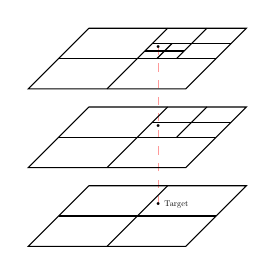
\begin{tikzpicture}
		\draw[dashed, color=red!40] (1.12, 0, 0.62) -- (1.12, 2, 0.62);
		
		\draw (0,0,0) -- (0,0,2) -- (2,0,2) -- (2,0,0) -- (0,0,0);
		\draw (1,0,0) -- (1,0,2);
		\draw (0,0,1) -- (2,0,1);
		
		\draw (0,1,0) -- (0,1,2) -- (2,1,2) -- (2,1,0) -- (0,1,0);
		\draw (1,1,0) -- (1,1,2);
		\draw (0,1,1) -- (2,1,1);
		\draw (1.5,1,0) -- (1.5,1,1);
		\draw (1,1,0.5) -- (2,1,0.5);
		
		\draw (0,2,0) -- (0,2,2) -- (2,2,2) -- (2,2,0) -- (0,2,0);
		\draw (1,2,0) -- (1,2,2);
		\draw (0,2,1) -- (2,2,1);
		\draw (1.5,2,0) -- (1.5,2,1);
		\draw (1,2,0.5) -- (2,2,0.5);
		
		\draw (1.25,2,0.5) -- (1.25,2,1);
		\draw (1,2,0.75) -- (1.5,2,0.75);
		
		\node at (1.12, 0, 0.62) {.};
		\node[scale=0.3] at (1.35, 0, 0.62) {Target};
		\node at (1.12, 1, 0.62) {.};
		\node at (1.12, 2, 0.62) {.};
	\end{tikzpicture}
\end{document}